\documentclass[runningheads]{llncs}

%---- Sonderzeichen-------%
\usepackage[ngerman]{babel}
%---- Codierung----%
\usepackage[utf8]{inputenc}
%\usepackage[latin1]{inputenc}
\usepackage[T1]{fontenc}
\usepackage{graphicx}
\usepackage{url}
\usepackage{llncsdoc}
%----- Mathematischer Zeichenvorrat---%
\usepackage{amsmath}
\usepackage{amssymb}
\usepackage{enumerate}
% fuer die aktuelle Zeit
\usepackage{scrtime}
\usepackage{listings}
\usepackage{subfigure}
\usepackage{hyperref}

\setcounter{tocdepth}{3}
\setcounter{secnumdepth}{3}

% -------------------------------------------------------------------------------------------------
% -------------------------------------------------------------------------------------------------

\mainmatter
\title{Universal Rendering}
\titlerunning{Universal Rendering}
\author{Julian Beck}
\authorrunning{Julian Beck}
\institute{Betreuer: Prof. Dr. rer. nat. Christian Zirpins}
\date{01.05.2019}
\begin{document}
\let\oldaddcontentsline\addcontentsline
\def\addcontentsline#1#2#3{}
\maketitle
\def\addcontentsline#1#2#3{\oldaddcontentsline{#1}{#2}{#3}}

% -------------------------------------------------------------------------------------------------

\begin{abstract}
  An dieser Stelle sollte später eine Kurzzusammenfassung stehen.
\end{abstract}

% -------------------------------------------------------------------------------------------------
\tableofcontents 
\newpage
% -------------------------------------------------------------------------------------------------

\section{Einleitung}
\label{sec:Einleitung}


\subsection{Anforderungen an eine Webanwendung}
\label{subsec:Anforderungen an eine Webanwendung}

\subsection{Terminologie}
\label{subsec:Anforderungen an eine Webanwendung}

% -------------------------------------------------------------------------------------------------

\section{Serverseitiges Rendering}
\label{sec:Serverseitiges Rendering}


\subsection{Serverseitiges Rendering mit Ajax}
\label{subsec:Serverseitiges Rendering mit Ajax}



Dies ist ein Zitat \cite{becker2008a}.
test\cite{IsomorphicApps}
test\cite{SearchFriendly}
test\cite{chen_chen_2016}


% -------------------------------------------------------------------------------------------------

\section{Clientseitiges Rendering}
\label{sec:Clientseitiges Rendering}
\begin{figure}[h]
  \centering
  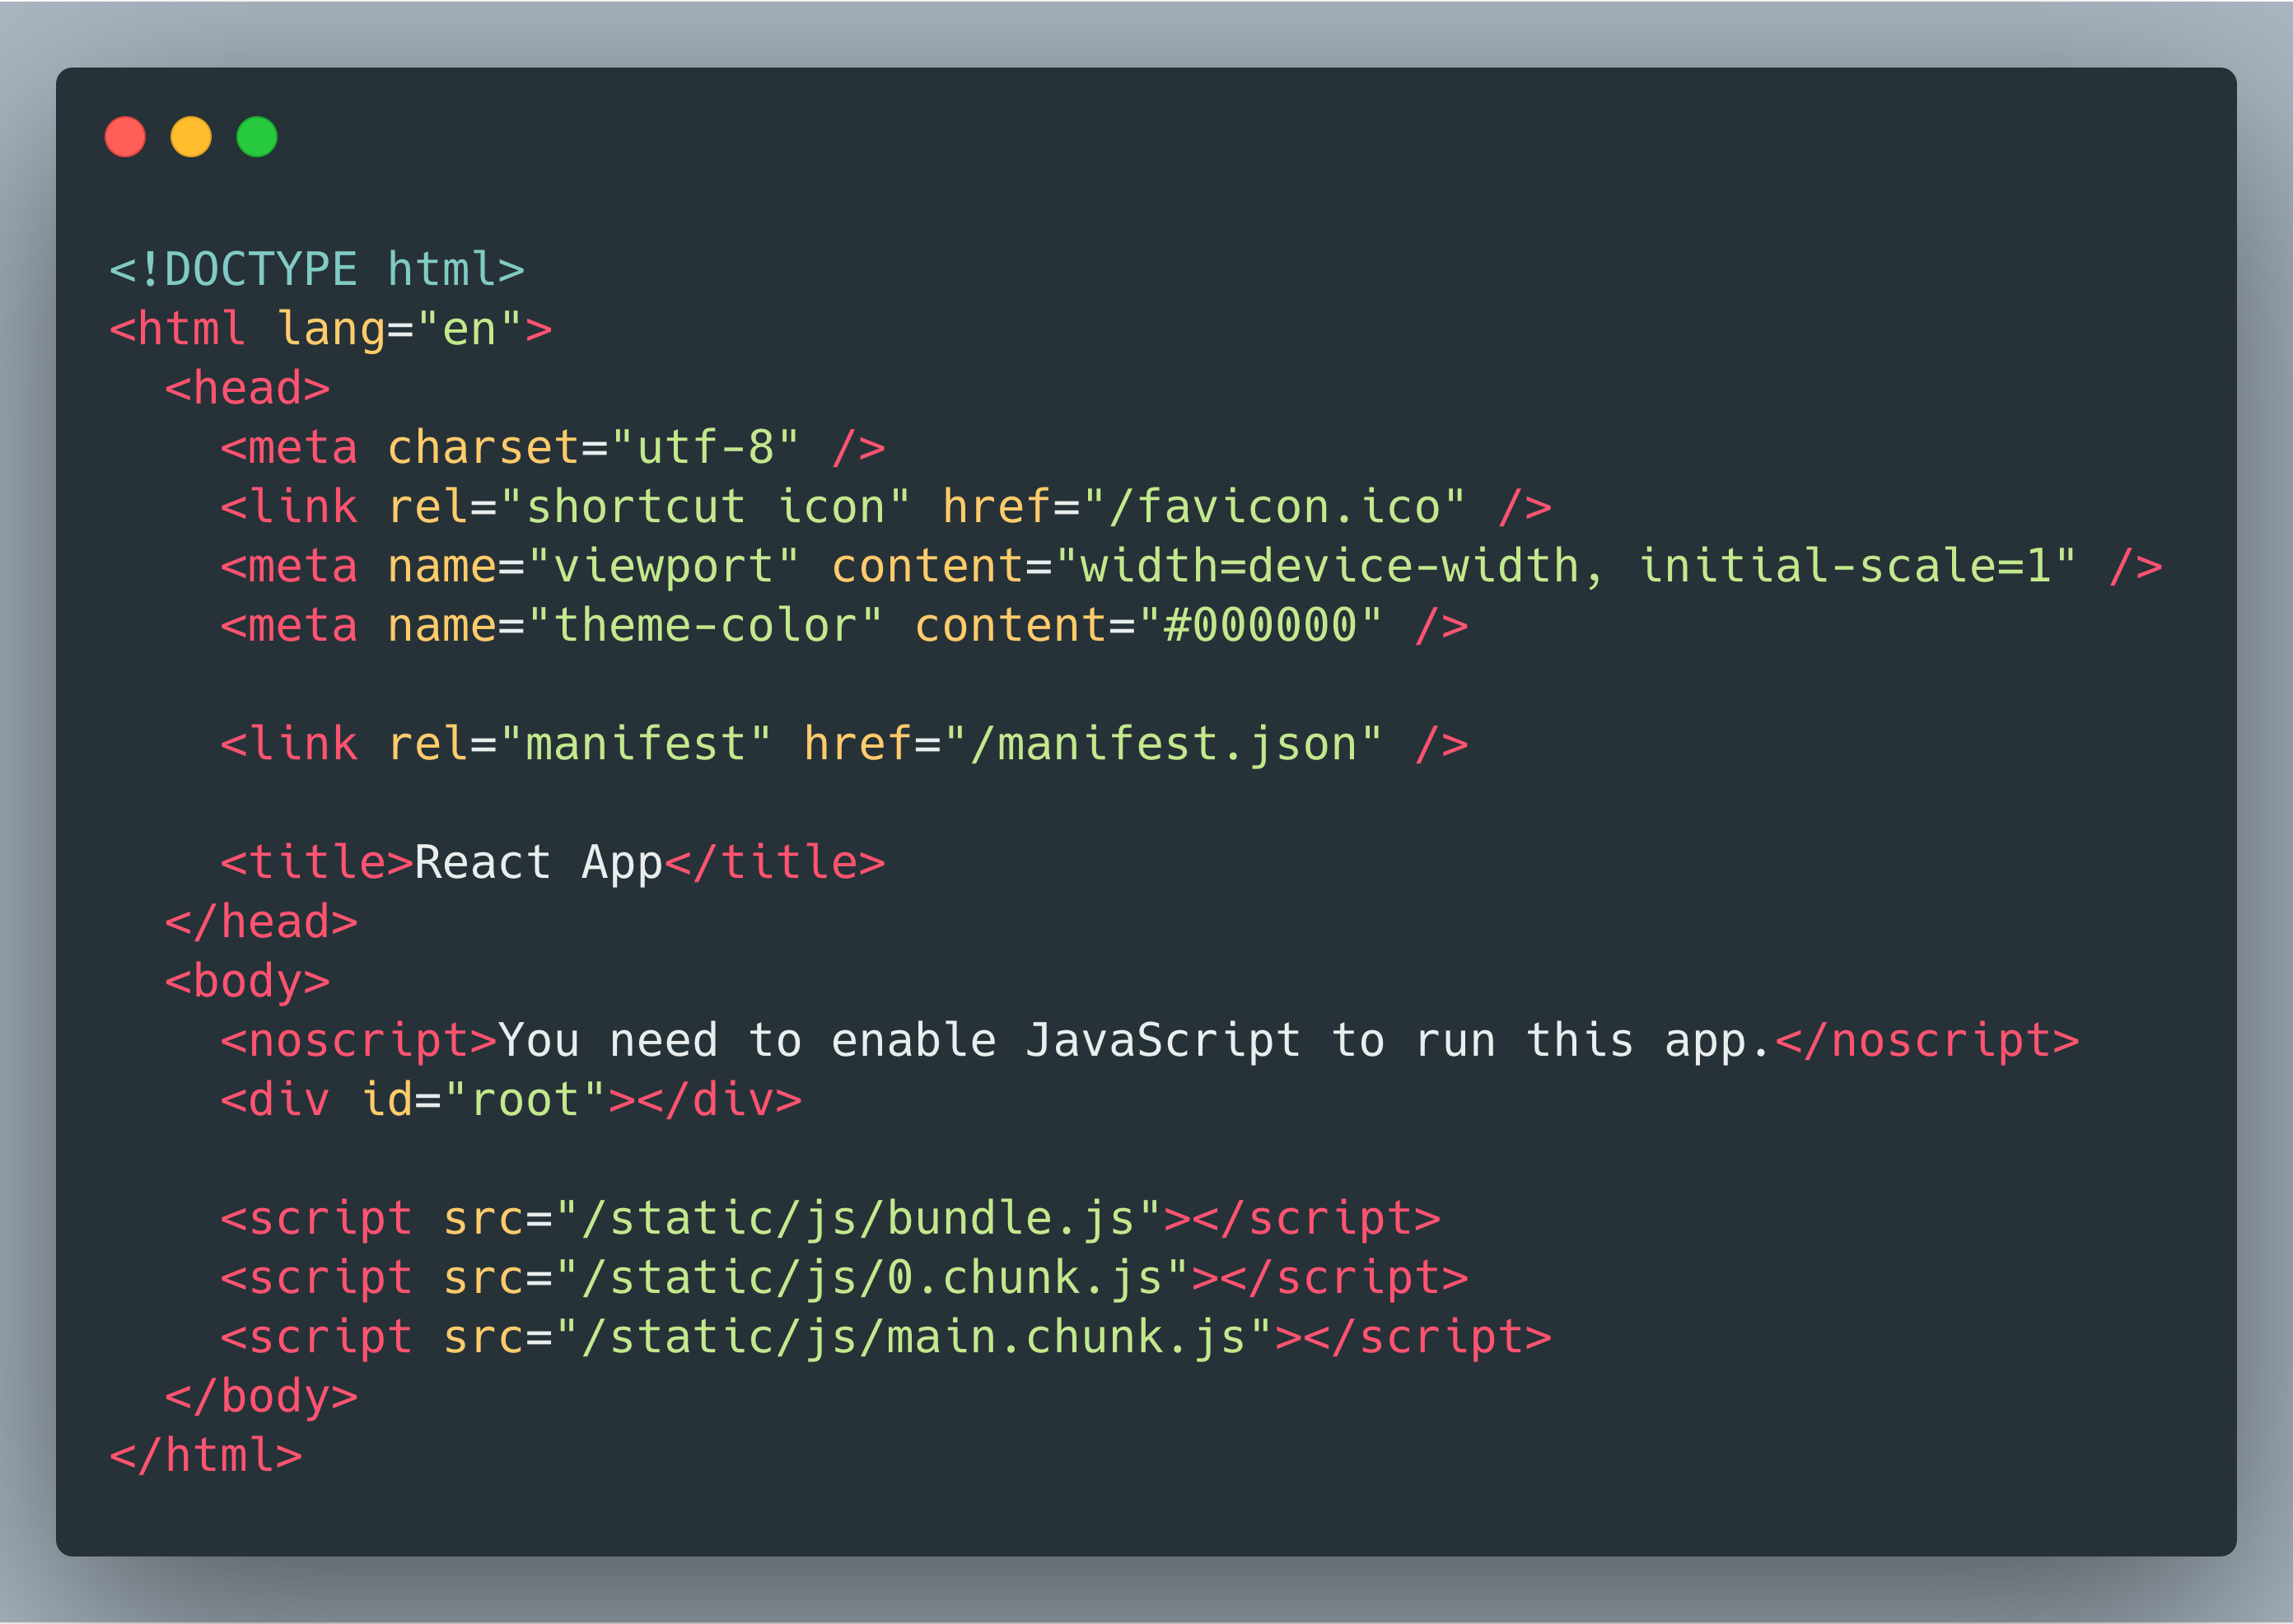
\includegraphics[width=12cm]{images/react-code}
  \caption{HTMl Dokument einer React Seite}
  \label{fig:iwilogo}
\end{figure}

% -------------------------------------------------------------------------------------------------

\section{Universal Rendering}
\label{sec:Universal Rendering}

\subsection{Isomorphic JavaScript}
\label{subsec:Isomorphic JavaScript}
\begin{figure}[h]
  \centering
  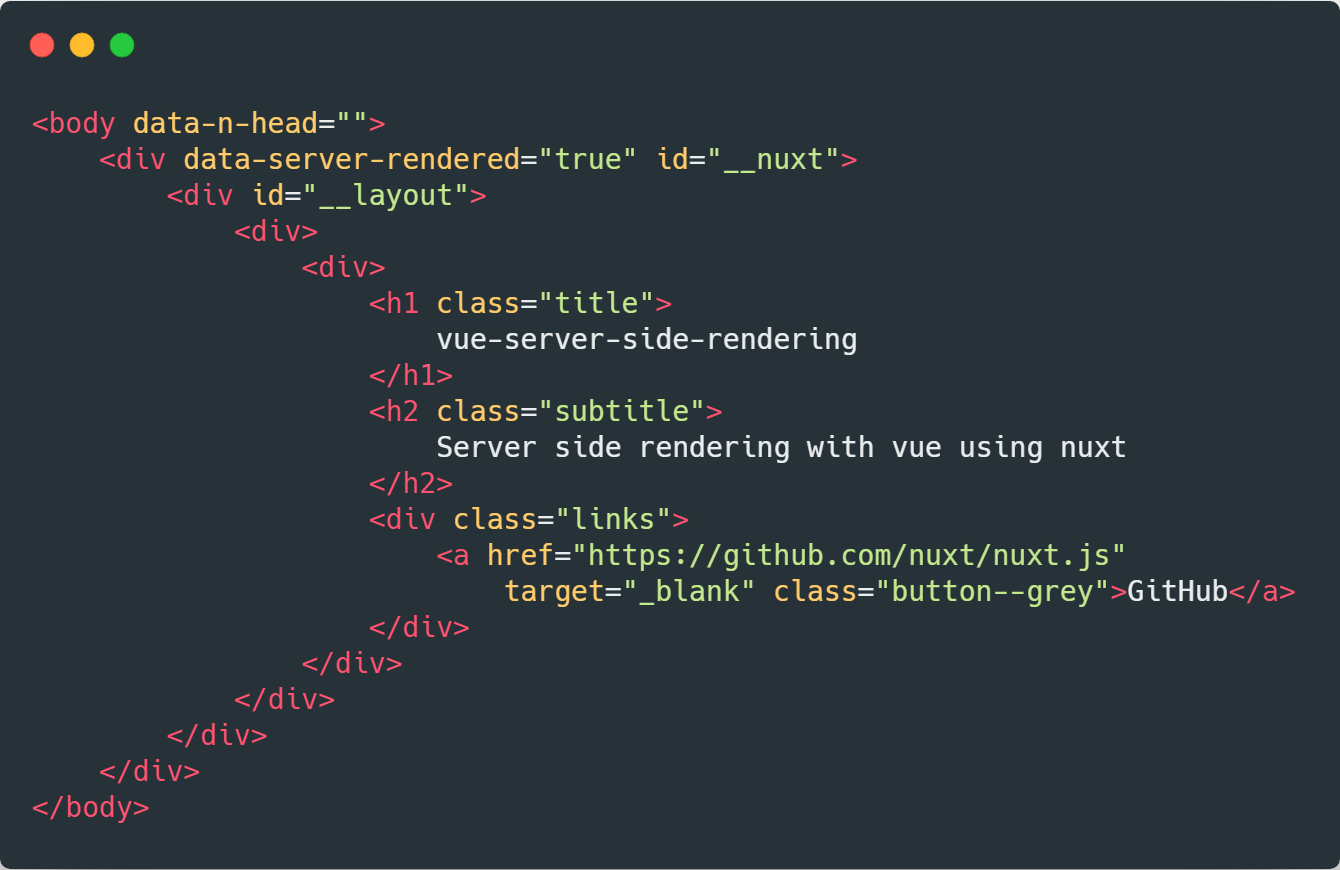
\includegraphics[width=12cm]{images/nuxt-body-first}
  \caption{HTMl Dokument einer React Seite}
  \label{fig:iwilogo}
\end{figure}

\subsection{Virtuelles DOM}
\label{subsec:Virtuelles DOM}

\subsection{Clientseitige Hydration}
\label{subsec:Clientseitige Hydration}

\subsection{Rendering Ablauf}
\label{subsec:Rendering Ablauf}

\subsection{Vorteile}
\label{subsec:Vorteile}

\subsection{Nachteile}
\label{subsec:Nachteile}

\subsection{Alternativen}
\label{subsec:Alternativen}
% -------------------------------------------------------------------------------------------------

\section{Frameworks}
\label{sec:Evaluation}

\subsection{React und Next.js}
\label{subsec:React und Next.js}

\subsection{Vue.js und Nuxt.js}
\label{subsec:Vue.js und Nuxt.js}

\subsection{Angular Universal}
\label{subsec:Angular Universal}


% -------------------------------------------------------------------------------------------------

\section{Universal Rendering in der Praxis}
\label{sec:Universal Rendering in der Praxis}


% -------------------------------------------------------------------------------------------------

\section{Fazit und Ausblick}
\label{sec:Fazit}


% -------------------------------------------------------------------------------------------------

% Normaler LNCS Zitierstil
%\bibliographystyle{splncs}
\bibliographystyle{itmalpha}
% TODO: Ändern der folgenden Zeile, damit die .bib-Datei gefunden wird
\newpage
\bibliography{literatur}

\end{document}
